\section{Background}
\label{sec:background}

This chapter introduces the three technical foundations on which the
remainder of this review depends: the transformer architecture that underlies
all reviewed models, the parameter-efficient fine-tuning primitives that
constitute the unit of adaptation, and the peer-to-peer network primitives
that provide the infrastructure vocabulary for the decentralisation
literature reviewed in later chapters. Readers familiar with these topics
may proceed directly to Section~\ref{sec:methodology}.

\subsection{Transformer Architecture}
\label{sec:background:transformer}

The transformer \cite{Vaswani2017} is a sequence-to-sequence architecture based
entirely on attention mechanisms, replacing recurrent and convolutional layers with
stacked blocks of multi-head self-attention and position-wise feed-forward networks.
Each transformer block applies two sub-layers: a multi-head attention (MHA) layer
that computes pairwise attention weights across sequence positions, and a feed-forward
network (FFN) that applies a two-layer MLP independently to each position. The
scaled dot-product attention function and multi-head attention are defined as:

\begin{equation}
\mathrm{Attention}(Q,K,V) = \mathrm{softmax}\!\left(\frac{Q K^T}{\sqrt{d_k}}\right) V
\label{eq:attention}
\end{equation}

\begin{equation}
\mathrm{MultiHead}(Q,K,V) = \mathrm{Concat}(h_1,\ldots,h_H) W^O,
\quad h_i = \mathrm{Attention}(Q W^Q_i, K W^K_i, V W^V_i)
\label{eq:mha}
\end{equation}

\begin{equation}
\text{FFN}(x) = W_2 \, \sigma(W_1 x + b_1) + b_2
\label{eq:ffn}
\end{equation}

Layer normalisation and residual connections wrap each sub-layer. Pre-trained
transformer backbones (GPT \cite{RadfordGPT22019,BrownGPT32020}, BERT \cite{Devlin2019}, T5 \cite{RaffelT52020}, LLaMA \cite{TouvronLLaMA2023}) capture rich linguistic and factual
knowledge in their weight matrices $\{W^Q, W^K, W^V, W^O, W_1, W_2\}$ through
large-scale self-supervised training, providing a universal feature extractor that
can be adapted to downstream tasks with minimal additional training. Devlin et al.~\cite{Devlin2019}
demonstrated that a BERT-style encoder pre-trained on masked language modelling
achieves state-of-the-art performance on 11 NLP benchmarks after lightweight
fine-tuning, establishing the pre-train--fine-tune paradigm as the dominant approach
in NLP.

\subsection{Parameter-Efficient Fine-Tuning Primitives}
\label{sec:background:peft}

Full fine-tuning of a pre-trained transformer updates every weight matrix in the
network for each downstream task, producing one full-size model copy per task.
For a GPT-3-scale model with 175 billion parameters, this is computationally and
storage-prohibitive at scale. PEFT methods address this by restricting updates to a
small structured subset of parameters while keeping the backbone frozen.

The three canonical PEFT approaches reviewed in this SLR are:
\begin{enumerate}
  \item \textbf{Bottleneck adapters} \cite{Houlsby2019}: compact modules inserted
    within each transformer layer that apply a down-projection, a non-linearity, and
    an up-projection to the layer's hidden representations (Equation~\ref{eq:bottleneck}).
  \item \textbf{Low-Rank Adaptation (LoRA)} \cite{Hu2022}: low-rank matrix products
    $\Delta W = BA$ added in parallel to the frozen attention weight matrices
    (Equation~\ref{eq:lora}).
  \item \textbf{Prefix tuning} \cite{LiLiang2021}: learnable continuous vectors
    prepended to the key--value representations at each layer to steer generation
    without weight modification.
\end{enumerate}

\begin{equation}
\mathrm{Adapter}(h) = W_{\mathrm{up}} \; \sigma( W_{\mathrm{down}} ( \mathrm{LayerNorm}(h) ) ) + h
\label{eq:bottleneck}
\end{equation}

\begin{equation}
h \gets h + \frac{\alpha}{r}\, x B A
\label{eq:lora}
\end{equation}

All three approaches produce a small, self-contained parameter delta (the \textit{adapter})
that encodes task-specific knowledge additive to the frozen backbone. This modularity
is the structural property that enables adapter exchange in a P2P setting: an adapter
can be transmitted independently of the backbone, and applied to any copy of that
backbone at inference time. Figure~\ref{fig:concept_peft_paradigm} illustrates 
this progression from full fine-tuning through per-task adapters to shared 
repositories, and Figure~\ref{fig:peft_adapter_types} compares the three 
canonical adapter structures at the module level.

\begin{figure}[H]
  \centering
  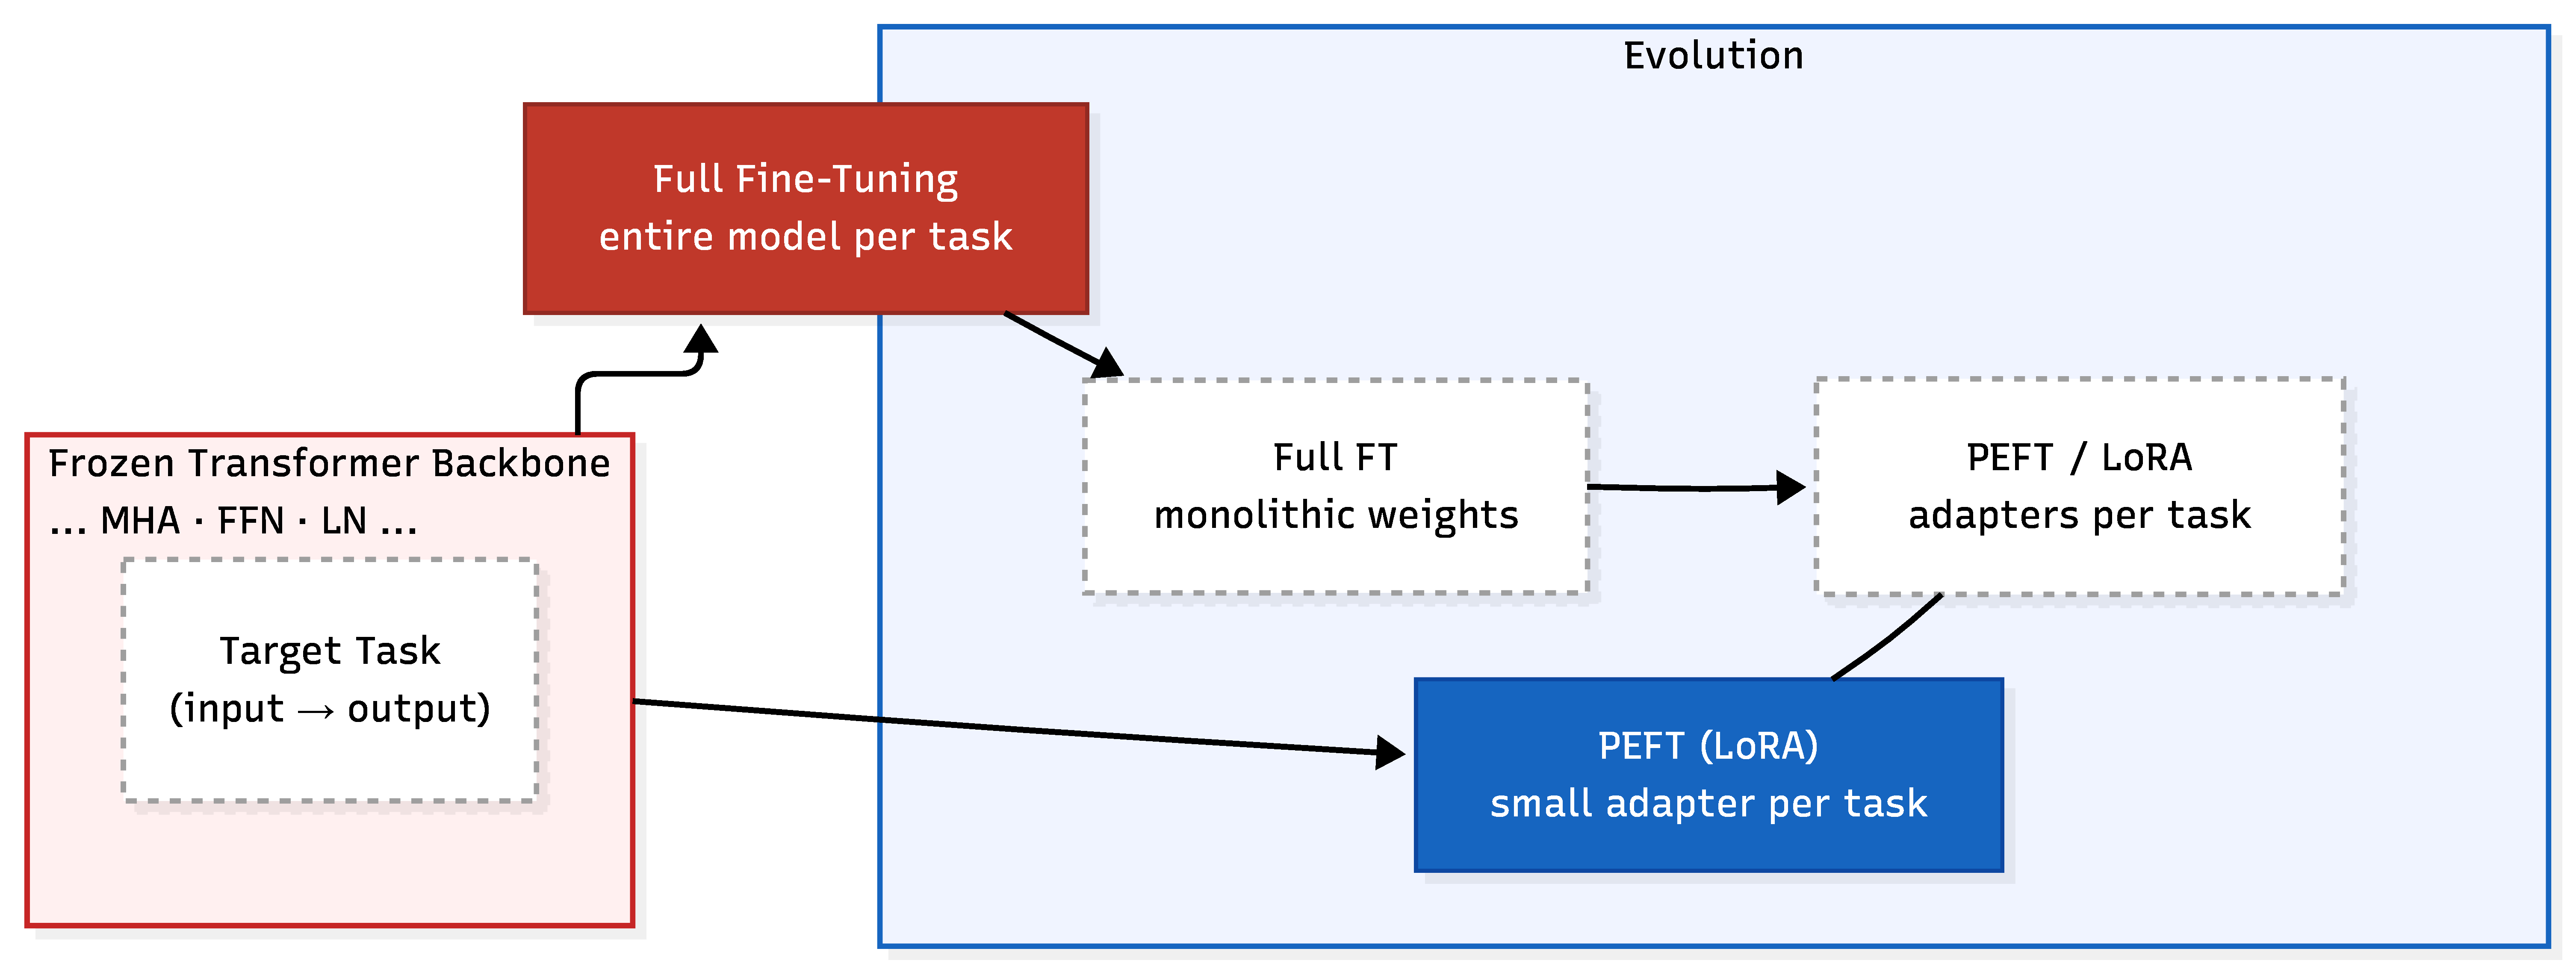
\includegraphics[width=0.65\linewidth]{figures/fig_concept_peft_paradigm.pdf}
\caption{Evolution of fine-tuning paradigms: from full fine-tuning of the
entire model, through parameter-efficient adapters trained per task, to
adapter exchange via shared repositories such as AdapterHub
\cite{Pfeiffer2020hub}.}
  \label{fig:concept_peft_paradigm}
\end{figure}

\begin{figure}[H]
  \centering
  % CREATE AN ORIGINAL FIGURE here (own drawing, no reproduction permission
  % needed): the three canonical adapter structures. Drop your PDF into
  % figures/ and replace the \fbox placeholder below with \includegraphics.
  \fbox{\parbox{0.85\textwidth}{\centering\vspace{1.6cm}
    \textit{Figure: Adapter structural types}\\[0.4em]
    \small(create original figure here)\vspace{1.6cm}}}
  \caption{Adapter structural types (own figure): (a) bottleneck adapter
    modules inserted into a transformer block; (b) LoRA low-rank matrices added
    in parallel to attention weights; (c) prefix tuning prepends learnable
    key-value vectors \cite{Houlsby2019, Hu2022, LiLiang2021}.}
  \label{fig:peft_adapter_types}
\end{figure}



\subsection{Peer-to-Peer Network Primitives}
\label{sec:background:p2p}

A peer-to-peer (P2P) network is a distributed system in which each participant
(peer) is both a client and a server: peers contribute resources (compute, storage,
bandwidth) to the network and consume resources from other peers, without any
centralised infrastructure. P2P networks are characterised by \textit{churn}
(peers may join and leave arbitrarily), \textit{heterogeneity} (peers differ in
hardware, bandwidth, and data), and \textit{no global state} (no single node has
visibility over the full network).

The \textbf{Distributed Hash Table (DHT)} is the primary data structure for
decentralised lookup in P2P systems. Maymounkov and Mazi{\`{e}}res~\cite{MaymounkovKademlia2002} introduced
Kademlia, a DHT in which each key--value pair is stored on the $k$ nodes whose
node IDs are closest to the key in XOR-metric space. Any peer can retrieve a
value for a given key by iteratively querying nodes whose IDs converge towards
the key, requiring at most $O(\log N)$ round trips in a network of $N$ peers.
Kademlia has been deployed in BitTorrent, Ethereum, and other large-scale P2P systems,
and its correctness and churn-tolerance are well-understood.

\textbf{Gossip protocols} provide a complementary mechanism for propagating information
in P2P networks without any routing infrastructure. In a gossip protocol, each peer
periodically selects a random neighbour and exchanges a subset of its local state;
over time, information spreads across the network in $O(\log N)$ rounds with high
probability \cite{OrmandyGossip2013}. Gossip protocols are inherently fault-tolerant
(peer churn merely slows convergence rather than breaking correctness) and
communication-efficient (each round requires only one peer-to-peer message).

These two primitives form the standard infrastructure layer of decentralised 
P2P systems: DHT-based lookup provides distributed indexing, and gossip-based 
propagation provides information dissemination. In file-sharing and blockchain
networks, for example, DHTs index resource locations while gossip protocols 
disseminate state updates across peers. Figure~\ref{fig:p2p_dht_lookup} illustrates 
the iterative convergence of a Kademlia lookup, and Figure~\ref{fig:p2p_gossip} 
shows how gossip-based propagation disseminates adapter metadata across the 
network in successive rounds.
% relabel slike dole
\begin{figure}[H]
  \centering
  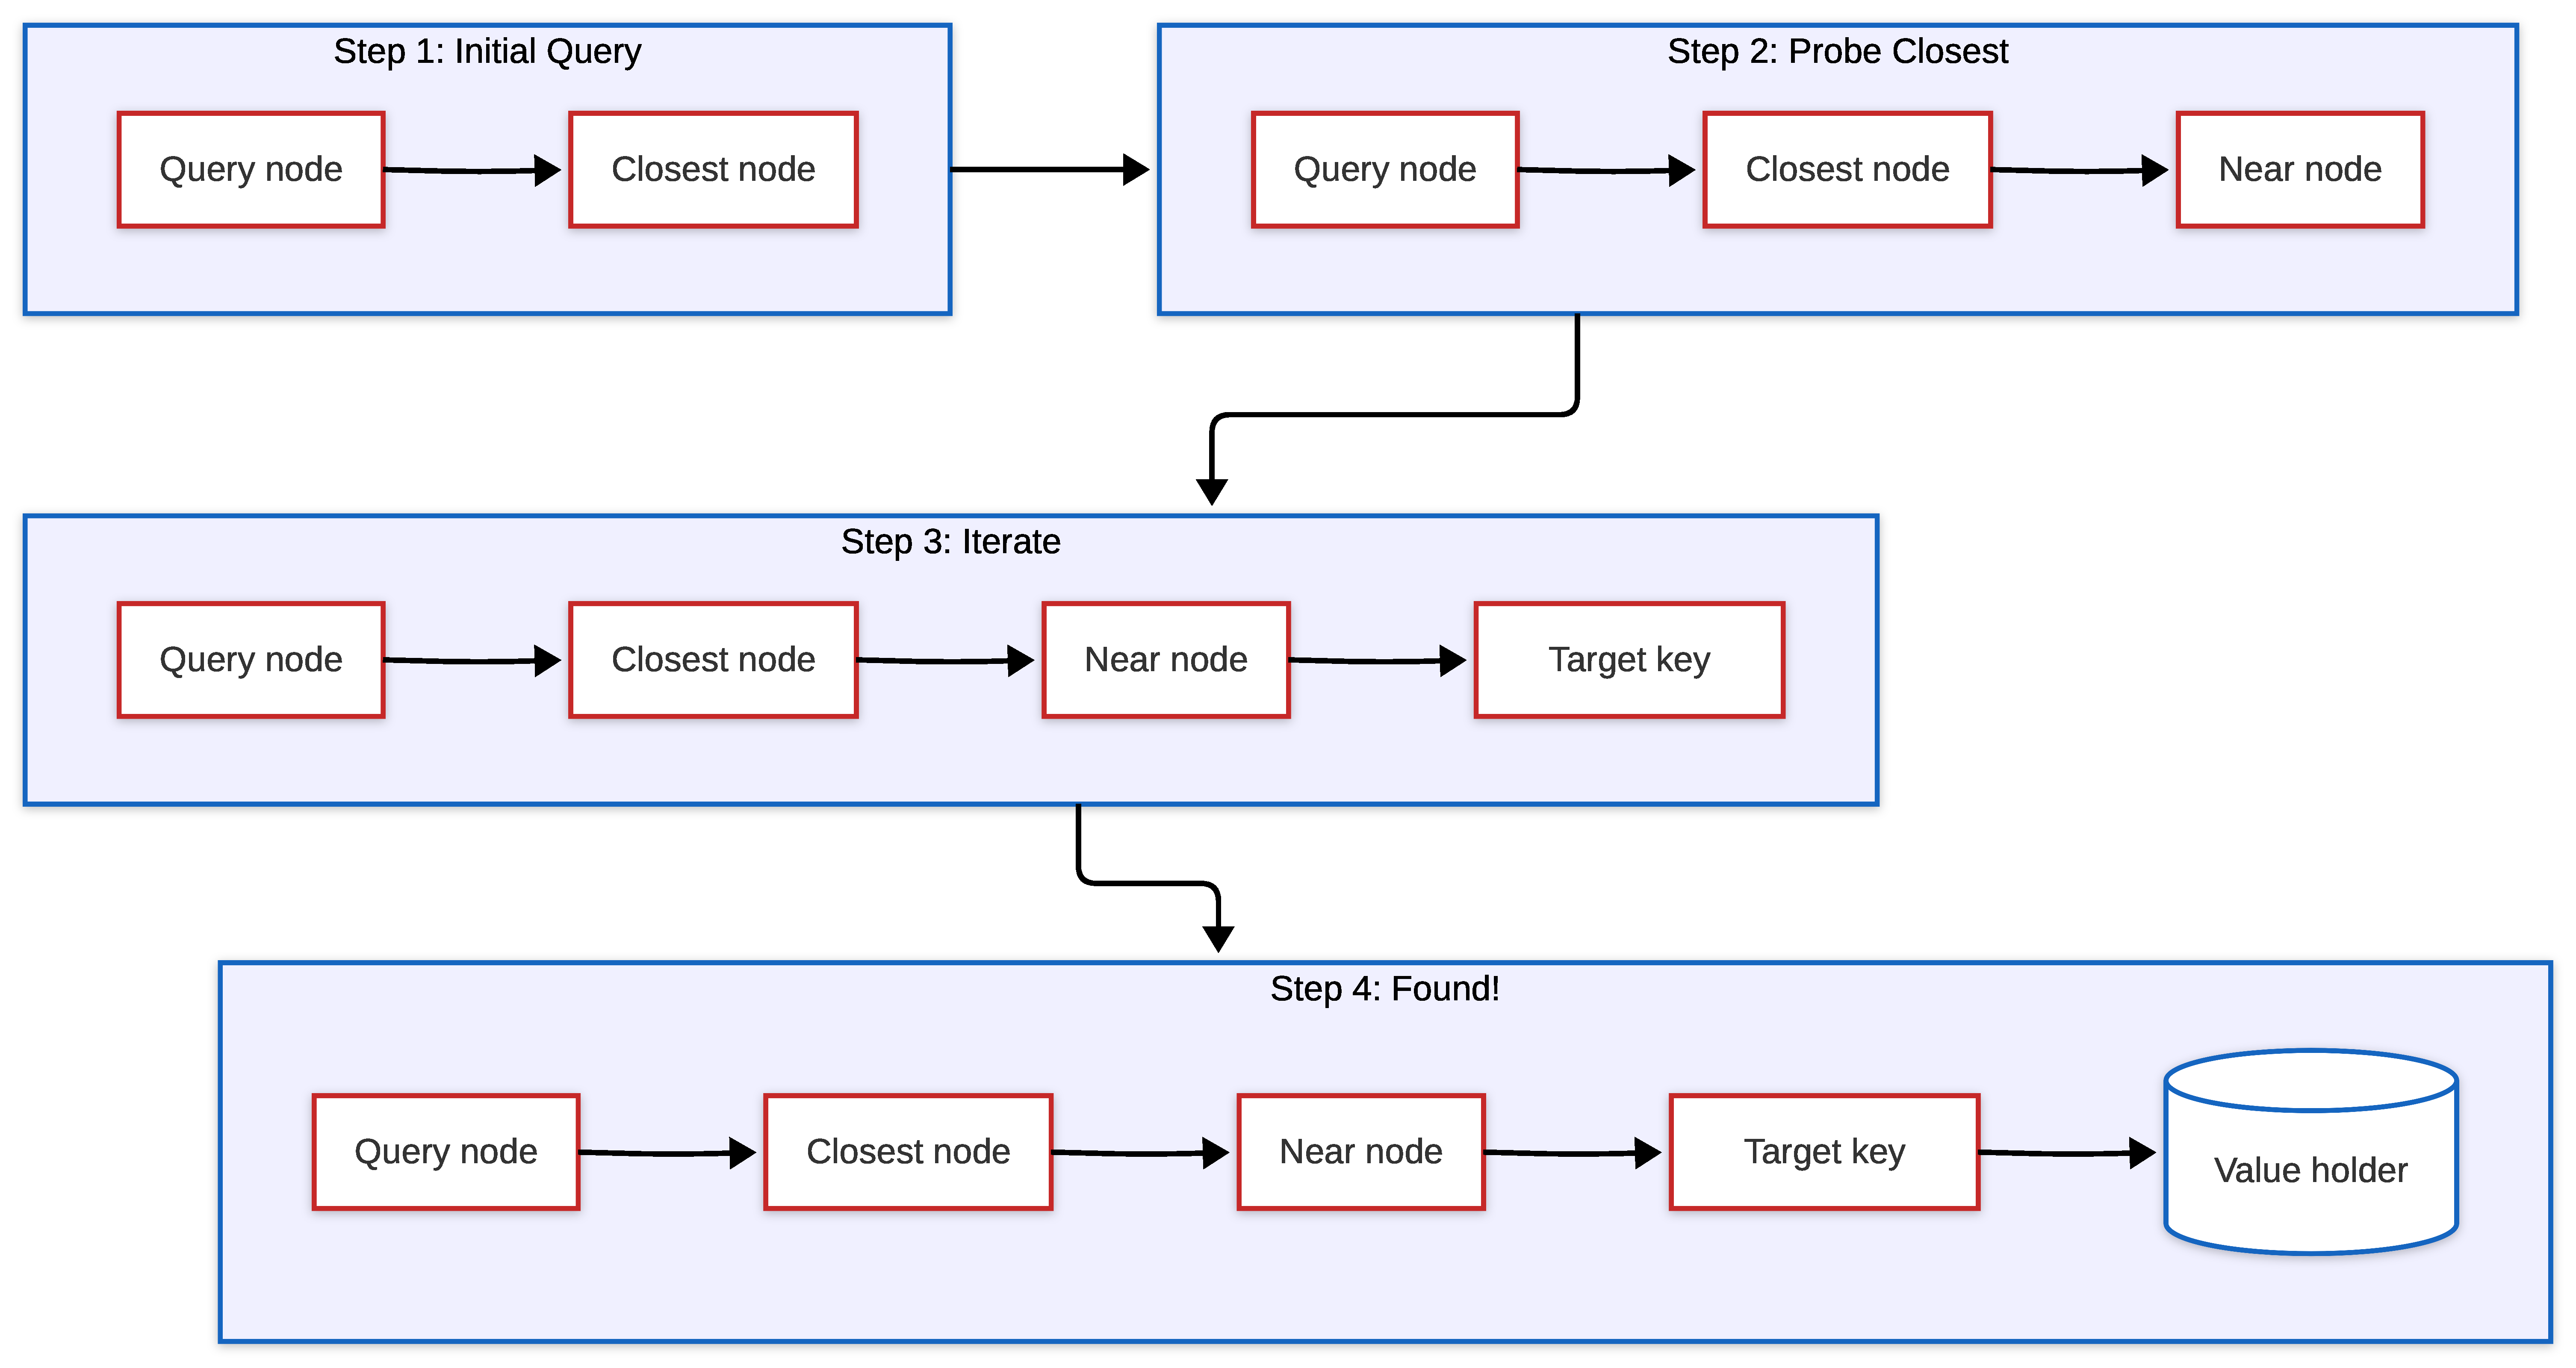
\includegraphics[width=1\linewidth]{figures/fig_p2p_dht_lookup.pdf}
  \caption{DHT lookup sequence: a query node iteratively probes increasingly close peers through XOR-metric routing until the target is reached.}
  \label{fig:p2p_dht_lookup}
\end{figure}

\begin{figure}[H]
  \centering
  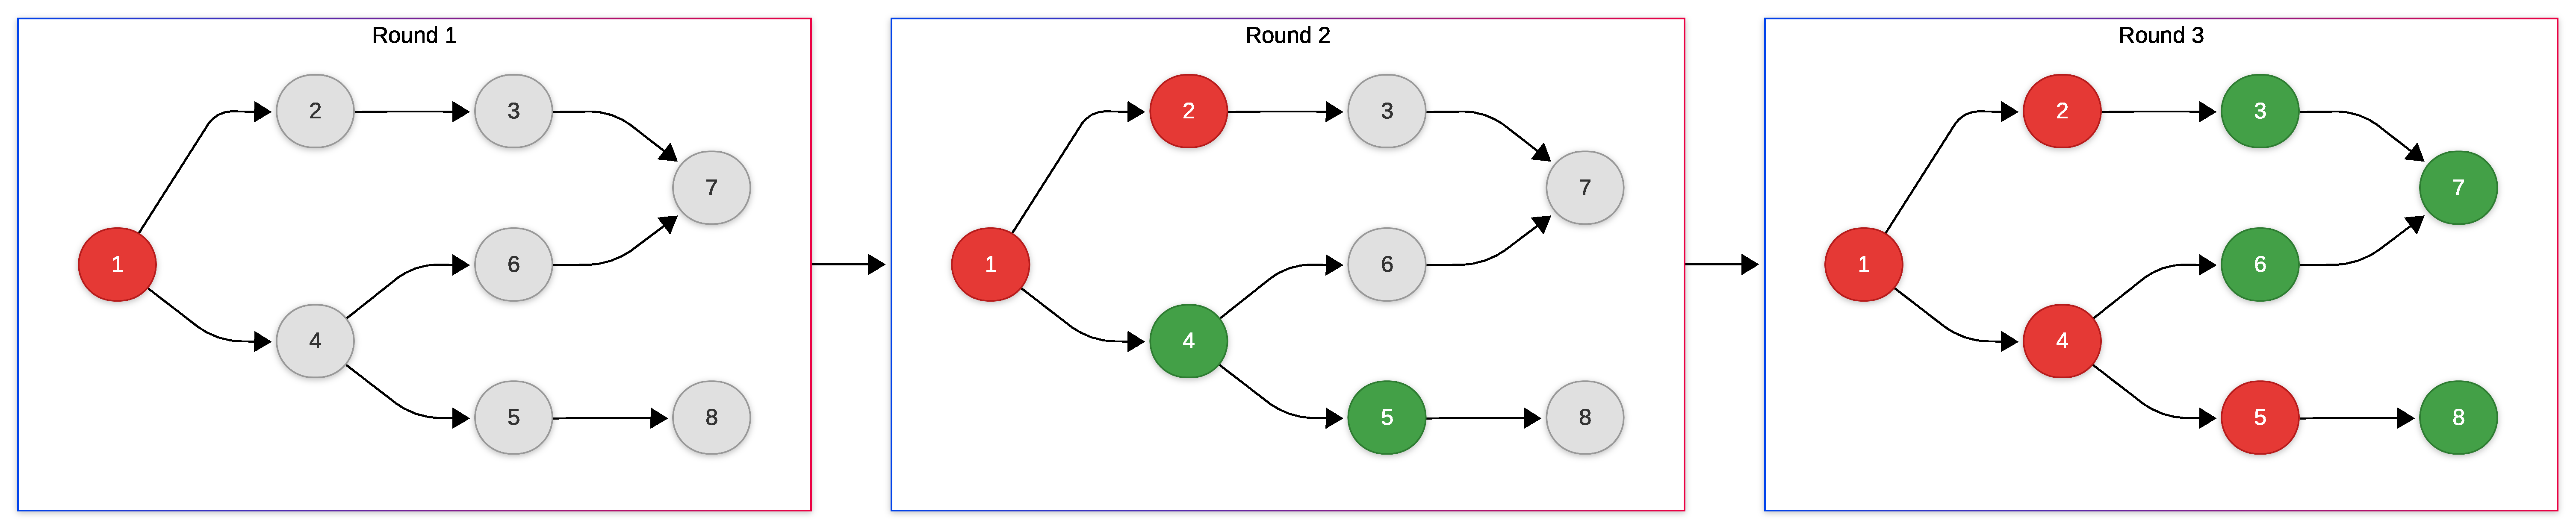
\includegraphics[width=1\linewidth]{figures/fig_p2p_gossip.pdf}
  \caption{Gossip propagation of adapter metadata: an infected peer spreads information to randomly chosen neighbours each round until the entire network is aware.}
  \label{fig:p2p_gossip}
\end{figure}

%\begin{figure}[H]
%  \centering
%  \includegraphics[width=0.65\linewidth]{figures/fig_concept_marketplace.png}
%  \caption{P2P exchange concept: autonomous nodes exchanging adapters over a DHT-based lookup with Kademlia-style %distributed storage.}
%  \label{fig:concept_marketplace}
%\end{figure}
